% --------------------------------------------------------------------
% LaTeX beamer slide example for Leiden slides
% Copyright LaTeX template: 2009-2010 by Joost Schalken
% --------------------------------------------------------------------

% ====================================================================
% Setup of slide environment
\batchmode % Do not display issues with package loading
\documentclass[t,11pt,aspectratio=169]{beamer}

% --------------------------------------------------------------------
% Load packages
\usepackage{booktabs}
\usepackage{graphicx}
\usepackage{tikz}
\usepackage{amsmath}
\usepackage{hyperref}
\usepackage{parskip}
\setlength{\parskip}{8pt}
\usetikzlibrary{calc,trees,positioning,arrows,chains,shapes.geometric,%
    decorations.pathreplacing,decorations.pathmorphing,shapes,%
    matrix,shapes.symbols}
\usepackage{listings}
\usepackage{array}

\lstset{
    tabsize=2,
    showspaces=false,
    showtabs=false,
    basicstyle=\ttfamily,
    showstringspaces=false,
    keywordstyle=\color{red},
    numbers=left,
    numberstyle=\small
}

% --------------------------------------------------------------------
% Beamer version theme settings
\usetheme[
    faculty=sciences,  % humanities, law, medicine, sciences, socialsciences
    lang=en,           % en, nl
    rmfont=pmn,
    logofont=fpi
]{leiden}

% Remove navigation symbols
\setbeamertemplate{navigation symbols}{}

% Better default font
\usepackage{iwona}
\usepackage[textfont={scriptsize,it}]{caption}
\setbeamerfont{caption}{size=\scriptsize}
\renewcommand*{\familydefault}{\sfdefault}
\captionsetup{labelformat=empty}




% --------------------------------------------------------------------
\def\liketitle#1{%
{\usebeamerfont{frametitle}\usebeamercolor[fg]{frametitle}%
\begin{flushleft}%
\vspace{-\baselineskip}% Cometic correction for space introduced by flushleft
#1\par
\end{flushleft}%
\vspace{-\baselineskip}% Cosmetic correction for space introduced by flushleft
}%
\vspace{0.75\baselineskip}%
}

% --------------------------------------------------------------------
\setbeameroption{hide notes}
%\setbeameroption{show notes}
%\setbeameroption{show notes on second screen}

% --------------------------------------------------------------------
\nonstopmode % Include issues with the slides


% ====================================================================
% Header settings
\def\lecturename{ETSC}
\subtitle{Gilles Ottervanger}
\date{\today}
\title{AutoML for Early Time Series Classification}
\author{Supervised by: Can Wang, Mitra Baratchi, Holger H. Hoos}
\institute{}
\subject{}
\def\footerbartext{Gilles Ottervanger \hspace{.2cm}\rule[-\dp\strutbox]{1pt}{1.2\baselineskip}\hspace{.2cm} AutoML for Early Time Series Classification}

% --------------------------------------------------------------------
\batchmode % Do not include issues with the package definitions
\begin{document}
\nonstopmode % Include issues with the slides


% ====================================================================

% --------------------------------------------------------------------
{
\setbeamertemplate{navigation symbols}{}
\begin{frame}[plain]
  \maketitle
\end{frame}
\addtocounter{framenumber}{-1}% don't count the title slide.
}

% --------------------------------------------------------------------
\begin{frame}[fragile]{Refresher: Early Time Series Classification}
\begin{columns}
\begin{column}{.45\textwidth}
\setlength{\parskip}{10pt}
\begin{itemize}[<+->]
    \item Processing as the data arrives.
    \item Classify before the full data is observed.
    \item Useful if the cost of data \alert{acquisition} is higher than cost of data \alert{processing}.
    \item Maximize \alert{accuracy} and \alert{earliness} simultaneously (Multi-Objective).
\end{itemize}
\end{column}
\begin{column}{.45\textwidth}
\vspace{-.5cm}
\uncover<1->{
    \begin{figure}
        \centering
        \begin{tikzpicture}
        \node[anchor=north west,inner sep=0] at (0,9) {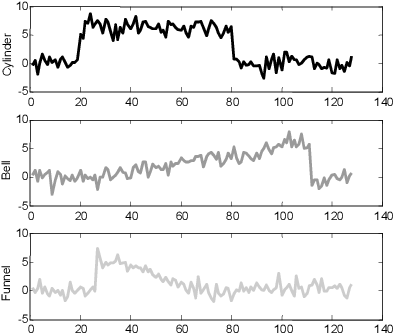
\includegraphics[width=\textwidth]{imgs/cylinderbellfunnel.png}};
        \draw[red,ultra thick,dashed] (.5,3.9) rectangle (2.5,8.9);
        \end{tikzpicture}
        \caption{Class examples from the \href{https://www.math.ucdavis.edu/~saito/publications/saito_phd.pdf}{CBF data set}\footnotemark}
        \label{fig:my_label}
    \end{figure}
}
\end{column}
\end{columns}
\footnotetext{N. Saito, ``Local Feature Extraction and Its Applications Using a Library of Bases'', Ph.D.Thesis (Advisor: Prof. Ronald R. Coifman), 1994.}
\end{frame}

% --------------------------------------------------------------------
\begin{frame}[fragile]{Previous work on EarlyTSC}
Task is split in two:
\begin{itemize}
    \item Classification
    \item Making the decision to stop processing more data and to \alert{trigger} the final class output.
\end{itemize}

Earliness-accuracy trade-off is user-defined beforehand (in most cases).

The current state-of-the-art consists of various methods based on different theoretical approaches (distance based, shapelets, RNNs).

\end{frame}

% --------------------------------------------------------------------
\begin{frame}[fragile]{Proposed approach: Multi-Objective CASH}
Embracing the multi-objective nature of EarlyTSC.

Combining the power of all state-of-the-art competitors.

Producing a Pareto set of non-dominated solutions (model configurations).

Letting the user make an informed decision.

\end{frame}

% --------------------------------------------------------------------
\begin{frame}[fragile]{Challenges of solving MO-CASH for EarlyTSC}
Defining the search space.

Preventing redundant training steps (exploit overlapping processing).

Efficiently searching the space (multi-objective Bayesian optimization).

Evaluating the resulting Pareto sets.
\end{frame}

% --------------------------------------------------------------------
\begin{frame}[fragile]{The search space:}
\tiny
\begin{table}[ht]
    \centering
    \begin{tabular}{l l l p{6.5cm}}
        \hline
         Algorithm & \multicolumn{2}{l}{Hyperparameter} \\ \hline \hline
         ECTS~\cite{Xing2011} & min. support & int & controls over-fitting \vspace{3px}\\ 
         EDSC~\cite{Xing2011a} & $minL$ & int & Minimum shapelet length\\
         & $maxL$ & int & Maximum shapelet length\\
         & $k$ & real & precision-recall trade off of shapelets\\
         & $\alpha$ & real & accuracy-earliness trade off \vspace{3px}\\ 
         RelClass~\cite{Parrish2013} & $\tau$ & real & Minimum reliability threshold \\
         & variant  & cat & Chebyshev, Quadratic, Box \vspace{3px}\\ 
         ECDIRE~\cite{Mori2016} & num classifiers & int & \\
         & $acc\_perc$ & real & desired level of accuracy as percentage of full data classification \vspace{3px}\\ 
         SR-CF~\cite{Mori2018}  & $\alpha$ & real & accuracy-earliness trade off \\ 
         & num classifiers & int & ~ \vspace{3px}\\ 
         SR-CF MO~\cite{Mori2019} &  $\gamma_{\{1,2,3\}}$ & real & internal parameters \\
         & num classifiers & int & ~ \vspace{3px}\\ 
         ECEC~\cite{Lv2019} & $\alpha$ & real & accuracy-earliness trade off \\ 
         & num classifiers & int & ~ \vspace{3px}\\ 
         TEASER~\cite{Schafer2019} & $v$ & int & Number of required consistent classifications \\
         & num classifiers & int & ~ \vspace{3px}\\ 
         EARLIEST~\cite{Hartvigsen2019} & $k$ & int & number of hidden dimensions\\
         & $\lambda$ & real & accuracy-earliness trade off\\
         & architecture & & complex search space on its own\\
         \hline
    \end{tabular}
    \caption{EarlyTSC algorithms and their hyperparameters}
    \label{tab:algs}
\end{table}
\end{frame}

% --------------------------------------------------------------------
\begin{frame}[fragile]{Candidate MO Bayesian Optimization implementation}
\href{https://gpflowopt.readthedocs.io/en/latest/notebooks/multiobjective.html}{GPFlowOpt}

Package based on GPFlow in turn based on TensorFlow...\pause 1.x \pause

I cannot be sure this is the state-of-the-art in MOBO. \pause

We might want ask someone who is more familiar with MOO.

\end{frame}

% --------------------------------------------------------------------
\begin{frame}[fragile]{Milestones}
\begin{tabular}{>{\small}r@{\hskip3pt} >{\small}l@{\hskip3pt} >{\small}l@{\hskip3pt} >{\small}l p{11cm}}
      Now&--& 15 & May   & Implementing (a subset of) the EarlyTSC algorithms with a common interface.\\
      15&--&31 & May   & Applying an out-of-the-box MO algorithm (e.g NSGA-II) and getting the first results.\\
      1&--&30& June & Improvements:\\
      &&&& ~~\llap{\textbullet}~~More efficient search (Bayesian optimization).\\
      &&&& ~~\llap{\textbullet}~~More efficient training.\\
      &&&& ~~\llap{\textbullet}~~Adding more EarlyTSC algorithms to the search space.\\
      1&--&15& July & Finishing thesis \\
\end{tabular}
\vspace{.7cm}\pause

My current challenge: I have a collection of EarlyTSC implementations. Should I try to reuse the existing code? Or re-implement completely?
\end{frame}

\begin{frame}[allowframebreaks]{References}
    \footnotesize
    \bibliographystyle{amsalpha}
    \bibliography{bibliography}
\end{frame}

\end{document}
